\documentclass{article}
\usepackage{tikz}
\usepackage{pgf-umlcd}
\begin{document}
\section{Ecuaciones diferenciales lineales de primer orden homog\'{e}neas}
Consideremos la ecuaci\'{o}n diferencial lineal homog\'{e}nea que describe el comportamiento 
del circuito el\'{e}ctrico de la figura
\begin{figure}[h]
\begin{center}
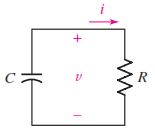
\includegraphics[width=6cm]{./images/02_Circuito_RC.jpg}
\caption{
Circuito RC sin fuente
}
\end{center}
\end{figure}
Utilizando la ley de corrientes de Kirchhoff  se obtiene la ecuaci\'{o}n diferencial
\begin{equation}
 C\frac{dv}{dt}+\frac{v}{R}=0
\end{equation}
Dividiendo entre $C$ obtenemos
\begin{equation}
 \frac{dv}{dt}+\frac{v}{RC}=0
 \label{EcuN}
\end{equation}
Para resolver la ecuaci\'{o}n utilizaremos un m\'{e}todo que consiste en sustituir la expresi\'{o}n $k_{0}e^{\lambda t}$ (donde $k_{0}\neq 0$ es una constante real) en todos los lugares de la ecuaci\'{o}n (\ref{EcuN}) en donde aparece $v$. Haciendo esto, se tiene
\begin{equation}
 \frac{d(k_{0}e^{\lambda t})}{dt}+\frac{k_{0}e^{\lambda t}}{RC}=0
\end{equation}
derivando y factorizando
\begin{eqnarray}
 \lambda k_{0}e^{\lambda t}+\frac{k_{0}}{RC}e^{\lambda t}&=&0\\
 (\lambda + \frac{1}{RC})k_{0}e^{\lambda t}&=&0\label{EcuNplus3}
\end{eqnarray}
dado que para todo $t\in R$, $e^{\lambda t}\neq 0$ (de hecho, si $\lambda\in R$, $e^{\lambda t}>0$ $\forall\,t\in R$). De (\ref{EcuNplus3}), concluimos que
\begin{equation}
 \lambda + \frac{1}{RC}=0
\end{equation}
de donde concluimos que $v(t)=k_{0}e^{-\frac{t}{RC}}$ es la soluci\'{o}n general de la ecuaci\'{o}n diferencial (\ref{EcuN}), (donde $k_{0}\neq 0$ es una constante real).
\section{Ecuaci\'{o}n diferencial lineal   homog\'{e}nea de segundo orden}
Consideremos el circuito RLC serie sin fuente de la siguiente figura
\begin{figure}[h]
\begin{center}
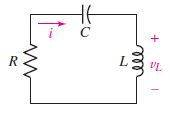
\includegraphics[width=6cm]{./images/CIRCUITO_RLC_serie.jpg}
\caption{
Circuito RLC sin fuente
}
\end{center}
\end{figure}
Suponiendo valores de $R$, $L$ y $C$ constantes, derivaremos a continuaci\'{o}n una ecuaci\'{o}n diferencial de segundo orden que describe el comportamiento del circuito de la f\/igura anterior. Dado que los tres elementos del circuito est\'{a}n conectados en serie, la corriente $i$ indicada para el capacitor, con la direcci\'{o}n adecuada es tambi\'{e}n la corriente en la inductancia y en el resistor. De la ley de voltajes de Kirchhoff, tenemos que
\begin{equation}
 v_{R}+v+v_{L}=0
 \label{EcuNplus7}
\end{equation}
donde $v_{R}$ es el voltaje entre las terminales de la resistencia, $v$ es el voltaje entre las terminales del capacitor, y $v_{L}$ es el voltaje entre las terminales del inductor. Utilizaremos el voltaje $v$ (del capacitor) como variable dependiente para nuestra ecuaci\'{o}n diferencial de segundo orden. La relaci\'{o}n entre el voltaje $v$ y la corriente $i$ es
\begin{equation}
 i(t)=C\frac{dv}{dt},
 \label{EcuNplus8}
\end{equation}
por lo que por la ley de Ohm, para $v_{R}$ usaremos la expresi\'{o}n
\begin{equation}
 v_{R}(t)=RC\frac{dv}{dt}.
 \label{EcuNplus9}
\end{equation}
Por \'{u}ltimo, como la relaci\'{o}n entre el voltaje $v_{L}$ en la inductacia y la corriente $i$ est\'{a} dada por
\begin{equation}
 v_{L}(t)=L\frac{di}{dt}.
 \label{EcuNplus10}
\end{equation}
Sustituyendo (\ref{EcuNplus8}) en (\ref{EcuNplus10}),
\begin{equation}
 v_{L}(t)=LC\frac{d^{2}v}{dt^{2}}.
 \label{EcuNplus10bis}
\end{equation}
Ahora, sustituyendo (\ref{EcuNplus9}) y (\ref{EcuNplus10bis}) en la ecuaci\'{o}n (\ref{EcuNplus7}),
\begin{equation}
 RC\frac{dv}{dt}+v(t)+LC\frac{d^{2}v}{dt^{2}}=0
 \label{EcuNplus11}
\end{equation}
Reacomodando los t\'{e}rminos de la ecuaci\'{o}n (\ref{EcuNplus11}) obtenemos
\begin{equation}
 LC\frac{d^{2}v}{dt^{2}}+RC\frac{dv}{dt}+v(t)=0
\label{EcuNplus12}
 \end{equation}
\section{Soluci\'{o}n de la ecuaci\'{o}n diferencial lineal homog\'{e}nea de segundo orden}
Para solucionar la ecuaci\'{o}n diferencial lineal
\begin{equation}
 LC\frac{d^{2}v}{dt^{2}}+RC\frac{dv}{dt}+v(t)=0
 \label{EcuNplus13}
\end{equation}
Propondremos una soluci\'{o}n de la siguiente forma
\begin{equation}
 v(t)=V_{1}e^{s_{1}t}+V_{2}e^{s_{2}t}
 \label{EcuNplus14}
\end{equation}
donde $V_{1}$, $V_{2}$, $s_{1}$, $s_{2}$ son constantes distintas de cero (no necesariamente n\'{u}meros reales, pueden ser n\'{u}meros complejos). Dado que ambos t\'{e}rminos en (\ref{EcuNplus14}), son de la forma
\begin{equation}
 v=K_{0}e^{st}
 \label{EcuNplus15}
\end{equation}
con $K_{0}$ y $s$ son dos constantes (no necesariamente n\'{u}meros reales). 
Sustituyendo (\ref{EcuNplus15}) en 
(\ref{EcuNplus13}) se tiene
\begin{equation}
LC\frac{d^{2}}{dt^{2}}\left(K_{0}e^{st}
\right)+RC\frac{d}{dt}\left(K_{0}e^{st}
\right)+K_{0}e^{st}=0 
\end{equation}
\begin{equation}
 \left(LCs^{2}+RCs+1\right)K_{0}e^{st}=0
\end{equation}
Por hipo\'{o}tesis $K_{0}\neq 0$ y para todo $s\neq 0$ se tiene que $e^{st}\neq 0$; por lo tanto
\begin{equation}
 LCs^{2}+RCs+1=0
 \label{EcuNplus16}
\end{equation}
En esta ecuaci\'{o}n, recordemos que los productos $LC$ y $RC$ son constantes. Bajo estas condiciones, como es bien sabido, la ecuaci\'{o}n (\ref{EcuNplus16}) tiene dos soluciones, estas pueden ser ambas reales, o bien, ambas complejas; y cuando son complejas, son complejas conjugadas. Ya sea que las ra\'{i}ces de la ecuaci\'{o}n (\ref{EcuNplus16}) sean reales o complejas, si denotamos esas ra\'{i}ces por $s_{1}$ y $s_{2}$, la soluci\'{o}n de la ecuaci\'{o}n diferencial (\ref{EcuNplus13}) se puede expresar como se plante\'{o} en la expresi\'{o}n (\ref{EcuNplus14}), es decir, de acuerdo concluimos
\begin{equation}
v(t)=V_{1}e^{s_{1}t}+V_{2}e^{s_{2}t}
 \label{EcuNplus17} 
\end{equation}
Dado que si $s_{1}$ y $s_{2}$ son ambas soluciones de (\ref{EcuNplus16}), entonces,
\begin{equation}
 LCs_{1}^{2}+RCs_{1}+1=0
 \label{EcuNplus18}
\end{equation}
y tambi\'{e}n
\begin{equation}
 LCs_{2}^{2}+RCs_{2}+1=0
 \label{EcuNplus19}
\end{equation}
Al sustituir (\ref{EcuNplus17}) en el lado izquierdo de (EcuNplus13) se llega a
\begin{equation}
 \left(LCs_{1}^{2}+RCs_{1}+1\right)V_{1}e^{s_{1}t}+\left(LCs_{2}^{2}+RCs_{2}+1\right)V_{2}e^{s_{2}t}=0
\end{equation}
dado que los t\'{e}rminos entre par\'{e}ntesis son ambos iguales a cero.
\end{document}
